\section{Social Weaver - Concrete Domain Level}\label{sowe-concrete}

\subsection{Social Weaver - Firefox Plugin} \label{sowe-firefox}
This section will briefly explain what technologies we use for firefox plugin development and describe in detail how the Social Weaver plugin is implemented.

\subsection{Firefox}
Firefox is a free web browser that has been released 2004 by the Mozilla Foundation\footnote{\url{www.mozilla.org}}. It is being multi-licensed under Mozilla Public License (MPL)\footnote{\url{http://www.mozilla.org/MPL/1.1/}}, GNU Lesser General Public License and GNU (LGPL)\footnote{\url{http://www.gnu.org/licenses/lgpl-3.0.de.html}} General Public License (GPL) \footnote{\url{http://www.gnu.org/licenses/gpl-3.0.html}}. 

The reasons why we chose Firefox as prototype environment are the high distribution of the browser and an easy extendability with plugins, extensions and so on.

\subsection{Firefox Plugin Development}
To improve readability of the coming section \ref{firefox_plugin_requirements} \nameref{firefox_plugin_requirements}, we will discuss some aspects from the Mozilla Add-on SDK (Version 1.13) \footnote{\url{https://addons.mozilla.org/en-US/developers/docs/sdk/latest}}. Readers who are not interested to much into technical detail can skip this section.

The Add-on SDK allows to create add-ons for the browser using the most common web technologies (like HTML, CSS, JavaScript, ...). Furthermore it provides a Low-Level-API and a High-Level-API set. The most important interfaces that are being used for our prototype are High-Level-Interfaces and will be explained in the following.

\begin{description}
\item Panel\\
A \emph{panel}\footnote{\url{https://addons.mozilla.org/en-US/developers/docs/sdk/latest/modules/sdk/panel.html}} is very flexible dialog window. Its appearance and behavior is specified by a combination of a HTML and a JavaScript file. Additionally a CSS file might be used to change the look even further. The limitations of a panel are the limitations of the mentioned technologies. 
A panel is meant to be visible temporary and they are easy to dismiss because any user interaction outside the 

\begin{figure}\centering
		
\includegraphics[width=8cm]{images/example-panel.png}
		\caption{An example for a \emph{panel} that shows a list of anntations}
		\label{example-panel}
\end{figure} 

We will use the \emph{panel} for getting user input, displaying information (like in screenshot \ref{example-panel}) and to integrate our social media web elements. 

\item Simple-Storage\\
This module\footnote{\url{https://addons.mozilla.org/en-US/developers/docs/sdk/latest/modules/sdk/simple-storage.html}} is an easy to use method to store basic properties (booleans, numbers, strings, arrays, ...) across browser restarts. 

With an operation like

\begin{lstlisting}
var ss = require("sdk/simple-storage");
ss.storage.myNumber = 41.99;
\end{lstlisting}

we store a number like an object and can it access just as easy like that. The price for such a simple usage is paid with high limitations. For instance searching is basically not possible. Nevertheless we can store an array and search the array. 

That is exactly the way how we store our annotations for our prototype. More details will be provided in the next section.

\item Page-Mod\\
The \emph{page-mod}\footnote{\url{https://addons.mozilla.org/en-US/developers/docs/sdk/latest/modules/sdk/page-mod.html}} module enables us to act in a specific context related to a web page. Then it becomes possible to attach JavaScripts to it and to parse or modify certain web page parts.

In our context we are going to use \emph{page-mod} to parse the HTML code to find elements that can server as anchors for annotations. And of course to find elements that are already annotated.

\item Widget\\
The module that is called \emph{widget} \footnote{\url{https://addons.mozilla.org/en-US/developers/docs/sdk/latest/modules/sdk/widget.html}} is simply an interface to the Firefox add-on bar\footnote{\url{https://developer.mozilla.org/en-US/docs/The_add-on_bar}}. It is possible to attach \emph{panels} and trigger operations by clicking the \emph{widget}. 

\begin{figure}[h!] \centering
		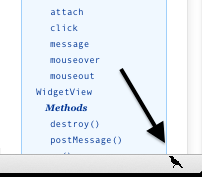
\includegraphics[width=7cm]{images/example-widget.png}
		\caption{Example for a widget serving as activation button}
		\label{example-widget}
\end{figure} 

We will use a widget to switch between different modes and to display an overview (see screenshot \ref{example-widget}). 

\item Self\\
\emph{Self}\footnote{\url{https://addons.mozilla.org/en-US/developers/docs/sdk/latest/modules/sdk/self.html}} provides access to add-on specific information like the Program ID\footnote{\url{https://addons.mozilla.org/en-US/developers/docs/sdk/latest/dev-guide/guides/program-id.html}}, which is important for an official distribution of the add-on. More meta information like the name or the version are accessible via the \emph{self} module. Also bundled external files are integrated by \emph{self}.

\item Notifications\\
This module\footnote{\url{https://addons.mozilla.org/en-US/developers/docs/sdk/latest/modules/sdk/notifications.html}} displays toaster\footnote{\url{http://en.wikipedia.org/wiki/Toast_(computing)}}-messages that disappear after a short time.

We use these to keep the user informed without bothering him to much with forcing him to dismiss trivial notifications.

\item Request\\
This simple to use but yet powerful module \emph{request}\footnote{\url{https://addons.mozilla.org/en-US/developers/docs/sdk/latest/modules/sdk/request.html}} lets us perform network requests. Once we create a \emph{Request} object we can specify whether it is a GET, PUT or POST request. These request types are specified by the REST standard so any web service that supports REST is able to interact with this module\cite{fielding2000principled}. The response from a server is directly accessible like a JavaScript object. 

We are going to use \emph{request} for our communication with our synchronization web service. 

\end{description}

\subsubsection*{JQuery}
\emph{jQuery}\footnote{\url{http://jquery.com/}} is a free JavaScript library under the MIT License\footnote{\url{http://www.mit.edu/}} that offers many functions for modifying DOM trees. It has been released 2006 in context of a BarCamp\footnote{\url{http://en.wikipedia.org/wiki/BarCamp}} in New York.

Even though this library is not a part of the Mozilla Add-on SDK it is being heavily used by it. Basically any operation that changes the HTML code (like changing the background color of web elements) is being reached with jQuery.

\subsection{Requirements for the Plugin}\label{firefox_plugin_requirements}
Let us recap what requirements we gathered in section \ref{browser_plugin} on the abstract domain level \cite{van2009requirements}:

\begin{enumerate}
\item Displaying and managing a comment box related to specific web elements
\item Managing several comment boxes without disturbing the view on original content
\item Communication to server application
\item Creating Anchors
\item Creating content in uniform sending format
\item Parsing content from uniform sending format
\item Identifying web elements across different user sessions
\end{enumerate}

In the following specialization we apply the abstract requirements to our environment which is the \emph{Mozilla Plugin Development SDK} \footnote{\url{https://addons.mozilla.org}}. 

\subsubsection{Display Management Requirement}
Obviously "Displaying and managing a comment box related to specific web elements" consists of multiple sub requirement that we need to distinguish. 

Before we are able to annotate something, we first of all need a function to select or recognize a web element the users cursor points to (check 1.1 in figure \ref{abstract2concrete-1}). \emph{Selecting} in this context means that we analyze the Document Object Model (DOM)\footnote{\url{http://www.w3.org/DOM/}} tree and retrieve its \emph{id} from the closest DOM ancestor. This is easy to implement using the function \emph{mouseenter} from the JavaScript \footnote{\url{https://developer.mozilla.org/en-US/docs/JavaScript}} library jQuery \footnote{\url{http://jquery.com/}}. 

Now that we have located a specific web element we may annotate our comment box. For reasons of flexibility and simplicity we just annotate a HTML window (check 1.2 in figure \ref{abstract2concrete-1}), where we inject an external comment box (but basically every HTML-code is going to work). The Mozilla SDK high-level APIs \footnote{\url{https://addons.mozilla.org/en-US/developers/docs/sdk/latest/modules/high-level-modules.html}} offer all necessary tools to insert a HTML box as a \emph{Panel}\footnote{\url{https://addons.mozilla.org/en-US/developers/docs/sdk/latest/modules/sdk/panel.html}}.

\begin{figure}\centering
		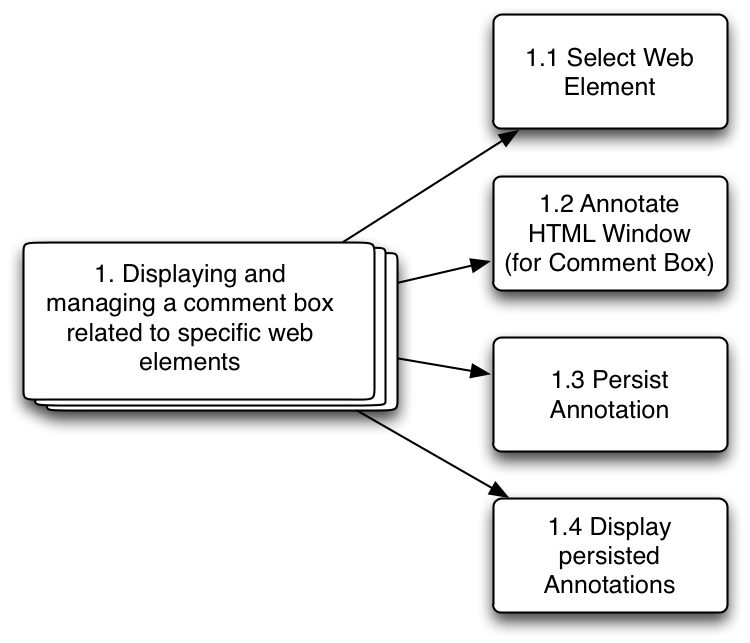
\includegraphics[width=10cm]{images/abstract2concrete-1.png}
		\caption{Partition of the first plugin requirement to sub requirements}
		\label{abstract2concrete-1}
\end{figure} 

The annotation anchors will be visible to the user in form of a colored background rectangle that we create by modifying the DOM tree. While the user moves the cursor above the web elements, while the plugin is activated, all elements that are annotatable will be marked with such a rectangle (see screenshot \ref{annotation-rectangle-sample}). 

\begin{figure} \centering
		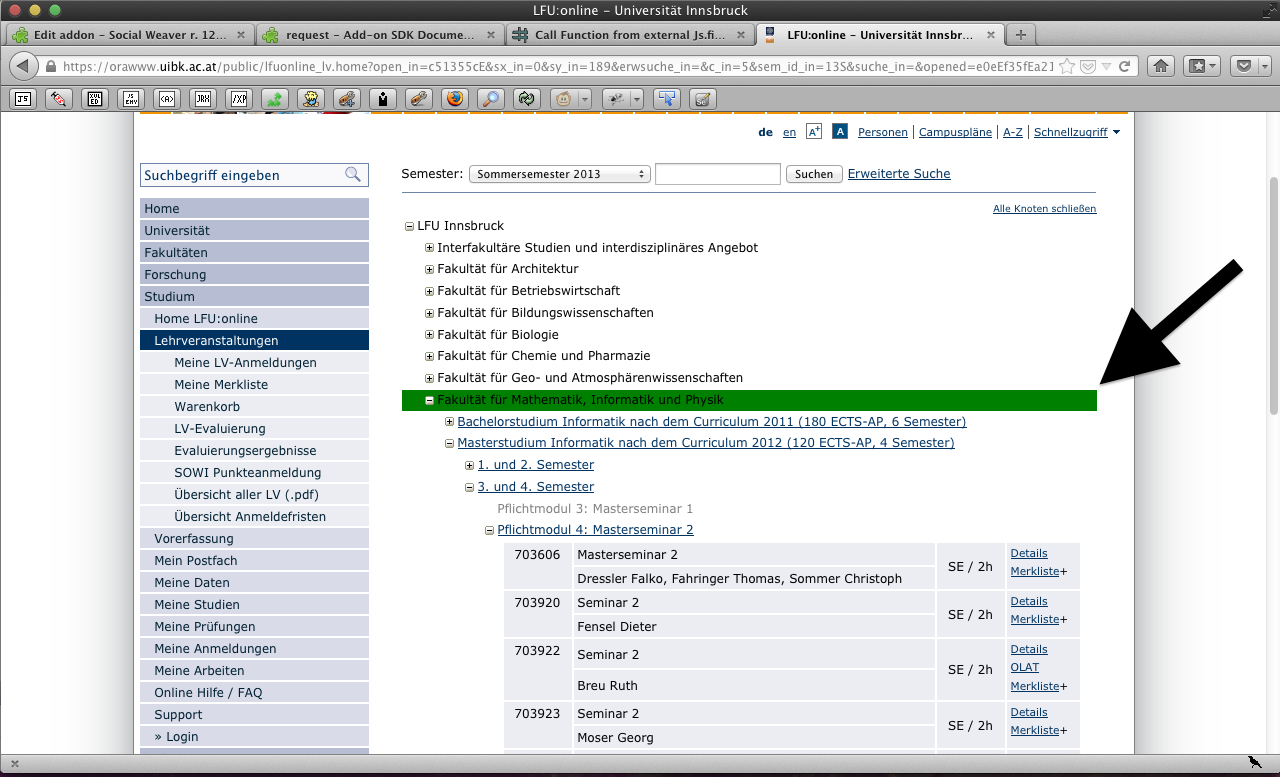
\includegraphics[width=12cm]{images/annotation-rectangle-sample.png}
		\caption{Rectangle shows that the underlying element is possible for annotation}
		\label{annotation-rectangle-sample}
\end{figure} 

Clicking on an element that is supported will append the above mentioned HTML panel. After that annotated elements will be marked with the rectangle. If the user clicks on such an element the already existing comment box will be reopened. 

To decouple our annotated data (like anchors, annotations, ...) from the actual synchronization, which will be covered later, we want to use a storing system that is also provided by the Mozilla SDK (see 1.3 in figure \ref{abstract2concrete-1}). The high level API \emph{simple-storage} \footnote{\url{https://addons.mozilla.org/en-US/developers/docs/sdk/latest/modules/sdk/simple-storage.html}} enables us to store all information we need and recall them. The synchronization mechanism should just modify this data set. All displaying procedures should be outside of server communication reach. 

The last sub requirement is to redisplay existing annotations (check 1.4 in figure \ref{abstract2concrete-1}) from our \emph{simple-storage}. Besides using the same techniques for drawing content and retrieving it from the storage we need to match the web page content to our saved annotations. For that we use a matcher instance that checks the DOM tree for IDs that we are already using. 

This is actually only trivial on a very simple basis. Let us assume that we will have more than one element attached to the same web element. Or we have different user sessions and/or include a workflow so that we need to distinguish the same element for different instances of the webpage. Than it becomes quite complicated to generate IDs that we can rely on. Nevertheless these issues will just affect the way we assign IDs to elements and how we retrieve them. The requirement 1.4 is just about matching existing IDs to a web page. 

As already mentioned we use a matcher that checks the DOM tree for IDs. In case we have an anchor in our \emph{simple storage} then we modify the web page HTML code similar as we did for requirement 1.1. Visual differences are that we do not modify the background of an element but generate an rectangle around it instead (see screenshot \ref{annotation-rectangle-sample2}). 

\begin{figure} \centering
		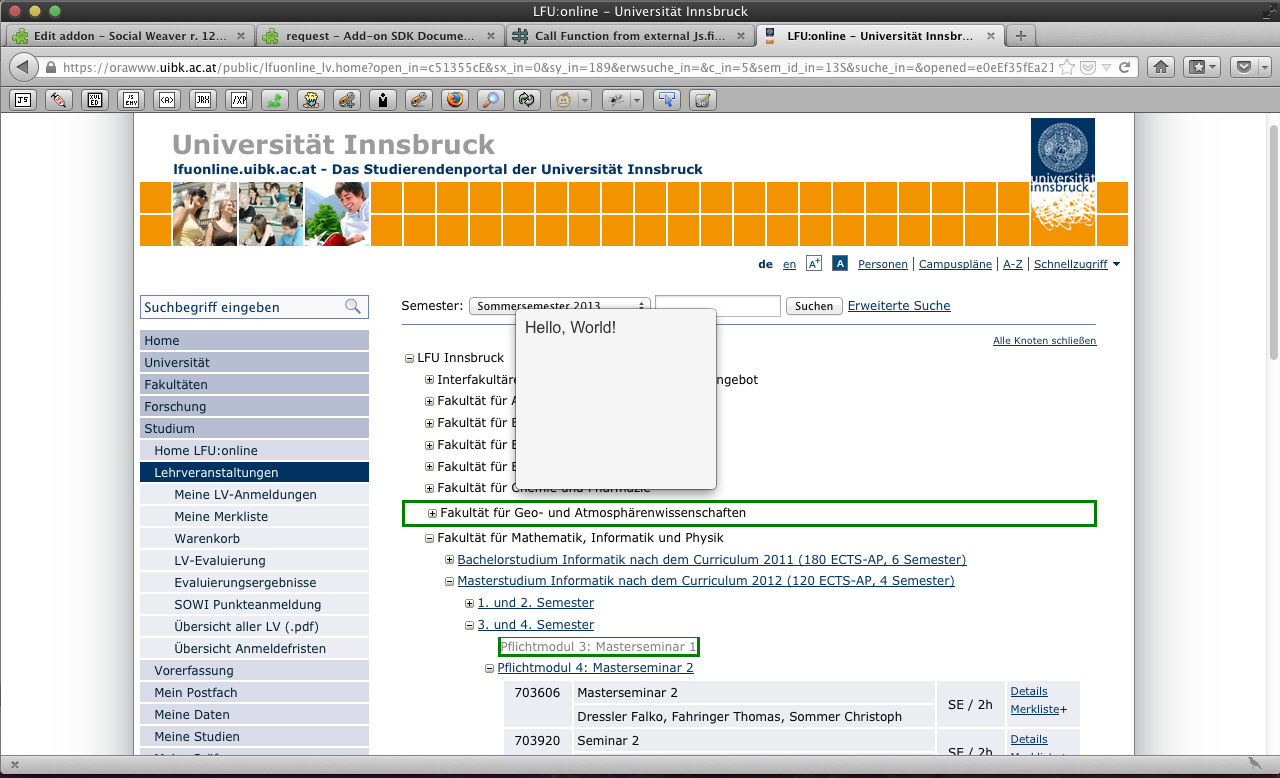
\includegraphics[width=12cm]{images/annotation-rectangle-sample2.png}
		\caption{Rectangle shows that the underlying element is possible for annotation}
		\label{annotation-rectangle-sample2}
\end{figure} 

This way we are able to show the user which elements are annotated. Of course without further information it is not obvious what is annotated exactly. What we need is a easy to access functionality so that the user can find out what the annotation is. 

For that reason we modify the above mentioned matcher class to generate a panel in case the user performs a \emph{mouseenter} operation. This panel should show a brief version of the attached social element. In our case it could be the name of the context the comment box is related or the names of the attendees (our example screenshot just print outs "Hello, World!" \ref{annotation-rectangle-sample2}). 

\subsubsection{Managing several comment boxes without disturbing the view on original content}
This requirement is not directly about functionality but should assure a positive user experience. It will be possible to attach annotations to nearly any element in a web application. This is a lot of potential additional footage. Nevertheless the user needs to be in the position to navigate like usually within the application. 

Fortunately we already had this in mind while working on the previous requirement.  Existing annotations are marked with a rectangle that is displayed around the element we use as anchor point (see screenshot \ref{annotation-rectangle-sample2}). This way is probably not beautiful but efficient in not disturbing the structure of the application beneath. 

\subsubsection{Communication to server application}
To share our comments or annotations with other users we will need a server side synchronization procedure. This section is only about the requirements that are related to the plugin side. (Details to the server side will be discussed in \nameref{server} \ref{server}.)

The first step to achieve this goal is to establish a communication between the plugin and a web service. For this purpose we are going to make use of the \emph{request} module from the Mozilla Add-on SDK. It provides an easy to use JSON\footnote{\url{http://www.json.org/}} and REST(\cite{fielding2000principled}) assistance. 

We split this into the following sub requirements:
\begin{description}
\item Plugin receives updates from server\\
What the plugin needs to know from the server is a set of Anchors. Those Anchors contain information like the author identification, a timestamp and of course the content.
(see \ref{creating_triplets}) 
So at this point we assume that our server will provide a set formatted in JSON. The plugin generates a request to retrieve this data. 
\begin{figure}
\begin{lstlisting}[numbers=left]
var sync = Request({
      url: 'http://localhost:9998/anchor',
      onComplete: function(response) {
        for(var i = 0; i<response.json.length; i++){
            var r = response.json[i];

            newAnchor = new Array(r.anchorURL, 
		r.ancestorId, r.anchorText);
            var newAnnotationText = r.annotationText;
            handleNewAnnotation(newAnnotationText, 
		newAnchor);
     };
   }
});
sync.get();
\end{lstlisting}
\label{anchor_sample_code}
\caption{Sample JavaScript code for retrieving JSON objects from a web service with a GET REST request}
\end{figure}

This goal is surprisingly simple to achieve. In the sample code \ref{anchor_sample_code} we just need to specify the URL of the web service and we are able to access the JSON objects right away exactly like JavaScript objects. Then we use the JSON objects to create an anchor entity and use the existing \verb| handleNewAnnotion(newAnnotationText, newAnchor)| method to store it in our \emph{simple-storage} list. 

Our prototype is a proof-by-concept system, therefore we keep the synchronization really simple. Instead of checking for new annotations and match them with the already existing data, we just rewrite our local plugin data set with a copy from the server. This technique could easily lead to corrupt and inconsistent data sets. But since the prototype is not meant to be used for confidential data or in any real world scenario at all - we will just take our risks.

\item Plugin sends updates to server\\
When a user creates a new annotation or modifies it - the plugin should send an update to the web service immediately. Again we will set up a method using the \emph{request} module. 
\end{description}

How the data format looks like and how we will parse incoming messages will be reviewed later (in the sections \ref{creating_triplets}, \ref{creating_content} and \ref{parsing_content}.)

\subsection{Social Weaver - Web Service}
The coming part will be about the implementation of the web service that provides interfaces for our previously built plugin.

\subsection{Used Technologies}
Before we disucuss our web service architecture we first of all will list the used technologies and give a brief explanation. Readers who are farmiliar with the following terms may skip this section. 
After pointing out the architecture, we will map our defined requirements to our implementation and explain how those are achieved.

\begin{description}
	\item Model View Controller (MVC)
	\item OpenJPA
	\item PostgreSQL
	\item RESTful Web Services
	\item JSON
\end{description}

\subsection{Web Service Architecture}
The web service is a common MVC architecture that uses JSON/RESTful interfaces. The persistence layer is connected to a PostgreSQL database using OpenJPA. 

Our main entities are the Anchor and SocialElement. The Anchor has been already discussed from the concept point of view. The entity contains all the parameters that are necessary for matching web elements. This set of parameters can differ from one web application to another. Additionally the Anchor entity contains an OID that defines the Anchor even across different user sessions. This way updates can be performed more easily without having to check for all parameters every time. Which would be hard especially in those cases where an unusual set of matching parameters is being used. To avoid this difficulty but to still keep all parameters related we generate a hash from a combination of all relevant parameters. This hash is used as OID. 
Besides that the Anchor holds a timestamp with information about the last modified date. We use this data for the synchronization procedure. 

The entity SocialElement is handled as a separate entity but from the concept persepective it is a part of the Anchor. Basically it works as a container for any kind of social content. Because our prototype will just provide a simple HTML inject, the SocialElement will contain an URL and a reference to the Anchor. But it will be extendable to hold data for native and more complex social element types. 

The entities are implemented as beans and therefore being directly persisted in the PostgreSQL database.

According to the MVC pattern there are also controllers for the entities that provides several interfaces that are accessible through the standard REST requests. 

\begin{figure}[h!] \centering
		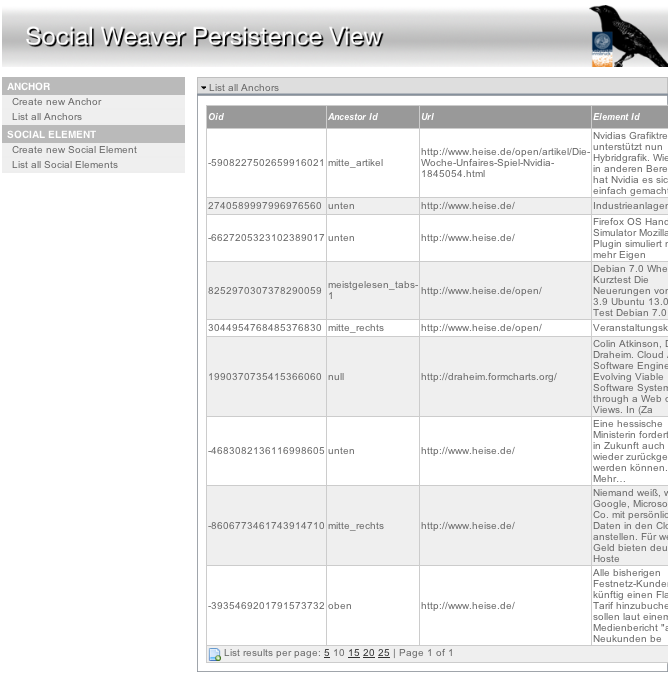
\includegraphics[width=9cm]{images/sowe-mvc-view-screenshot.png}
		\caption{Screenshot from Social Weaver Persistence Web View}
		\label{sowe-mvc-view-screenshot}
\end{figure} 

The View from our Model View Controller architecture is a web view that allows the user to check the content manually (see Figure \ref{sowe-mvc-view-screenshot}). This is just a pleasent side feature and not related to our Social Weaving use cases and for that reason this part should be discussed no further.


\subsection{Requirements for the Web Service}
In section \ref{Social Weaver - Server Application} we defined the following requirements for the web service:

\begin{enumerate}
	\item Offer service that receives messages from plugin-clients
	\item Synchronization for requests from different user-session
	\item Persist updates into a database
	\item Keep the server application independent to weaved-into web application
	\item Parse incoming messages
	\item Create outgoing messages
\end{enumerate}

\subsubsection{Offer service that receives messages from plugin-clients}
Cleary we accomplish this requirement with the RESTful web service interfaces. The messages that we transmit are the Anchor information right away. 


\subsubsection{Synchronization for requests from different user-session}

\subsubsection{Persist updates into a database}

\subsubsection{Keep the server application independent to weaved-into web application}

\subsubsection{Parse incoming messages}

\subsubsection{Create outgoing messages}
